\section{Simulations and Measurements of the MKI with 15 Screen Conductors}

To begin an analysis of the heating of the MKIs, and to verify the use of simulations as a tool for evaluating different designs of the MKI impedance reduction methods it was important to measure an existing MKI configuration as a benchmark. Due to the expected low beam coupling impedance of the MKI even with 15 screen conductors (on the order of 100$\Omega$ longitudinal beam coupling impedance) it was decided to do the measurements using the resonant coaxial wire method, described in Sec.~\ref{sec:reson-coax-meth}. This method limits the frequency resolution of the measurements ($\Delta{} f = c/ \Delta \lambda = c/2L_{device} \approx 40MHz$ where $c$ is the speed of light and $L_{device}\approx 3.5m$ is the length of the MKI in it's vacuum tank), but the added accuracy in this measurement is considered appropriate in this case.

The measurements were carried out on a fully assembled MKI inside it's vacuum tank, with a beam screen housing 15 tapered screen conductors. For the single wire measurements a copper wire of radius 0.5mm was placed in the central beam pipe, suspended on a vacuum flange modified to take a Sucobox connection allowing a capacitor housed in a seperate sucobox to be attached to the connecting box. To displace the wire for displaced single wire measurements, a pair of nylon screws (one at each flange) were used to physically displace the wire. Displacements were taken at 3mm intervals in both the vertical and horizontal planes, between -9mm and +9mm displacement.

For the two wire measurements, two wires were suspended in the device, seperated by 7mm. The wires were connected to a single VNA, each connection run through a 180$^{\circ}$ hybrid to generate the appropriate phase difference between the two. The experimental setup for the two wire measurements is shown in Fig.~\ref{fig:mki-meas-two-wire}.

The VNA is calibrated using an 8532E calibration kit, using an IF bandwidth of 1kHz. 2000 equally space data points are used over a frequency range of 1MHz-2GHz. The Q factors and resonant frequencies of the resonant modes are calculated using a peak finding algorithm on the VNA, and the conductive losses due to the copper wire calculated analytically and compensated for.

The simulations of the MKI are carried out using CST Particle Studio, a time domain simulation code. A simplified model of the magnet is created, shown in Fig.~\ref{fig:mki-simulation-model}. An integrated wakelength of 15m is used in the simulations, and a simulated bunch of a gaussian profile with $\sigma_{z}=$45mm used. A half model is used for displacements of the source/integration path in the vertical axis due to the symmetry plane in the y-z plane, giving a mesh count of $\approx$ 16 million for vertically displaced simulations and $\approx$ 16 million for horizontally displaced simulations. To acquire the dipolar and constant impedance terms, the source signal is displaced whilst the path of integration is kept on axis. The linear variation in the resulting impedance can be seen to be the dipolar term and the constant impedance the constant term. Similarly for the quadrupolar term the source signal is kept on axis and the 



\begin{figure}
\begin{center}
\includegraphics[width=0.5\textwidth]{LHC_MKI/figures/mki-two-wires.png}
\end{center}
\label{fig:mki-meas-two-wire}
\caption{The measurement setup for the two wire measurement setup. The 180$^{\circ}$ hybrid can be seen on top of the vacuum flange.}
\end{figure}

\begin{figure}
\begin{center}
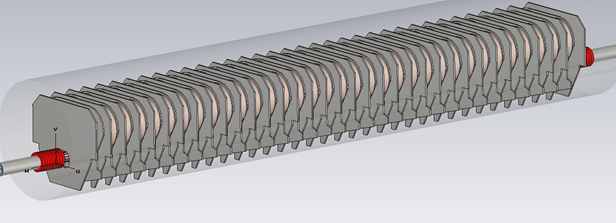
\includegraphics[width=0.5\textwidth]{LHC_MKI/figures/simulation-model-mki-15.png}
\end{center}
\label{fig:mki-simulation-model}
\caption{The simulation model of the LHC injection kickers implemented in CST Particle Studio.}
\end{figure}


The results for the measurements be seen in the following figures:
\begin{enumerate}
\item{Fig.~\ref{fig:mki-15-longitudinal} the longitudinal impedance}
\item{Fig.~\ref{fig:mki-15-horz-dipolar} the horizontal dipolar impedance}
\item{Fig.~\ref{fig:mki-15-vert-dipolar} the vertical dipolar impedance}
\item{Fig.~\ref{fig:mki-15-quadrupolar} the quadrupolar impedance}
\item{Fig.~\ref{fig:mki-15-constant} the constant transverse impedance}
\end{enumerate}

\begin{figure}
\begin{center}
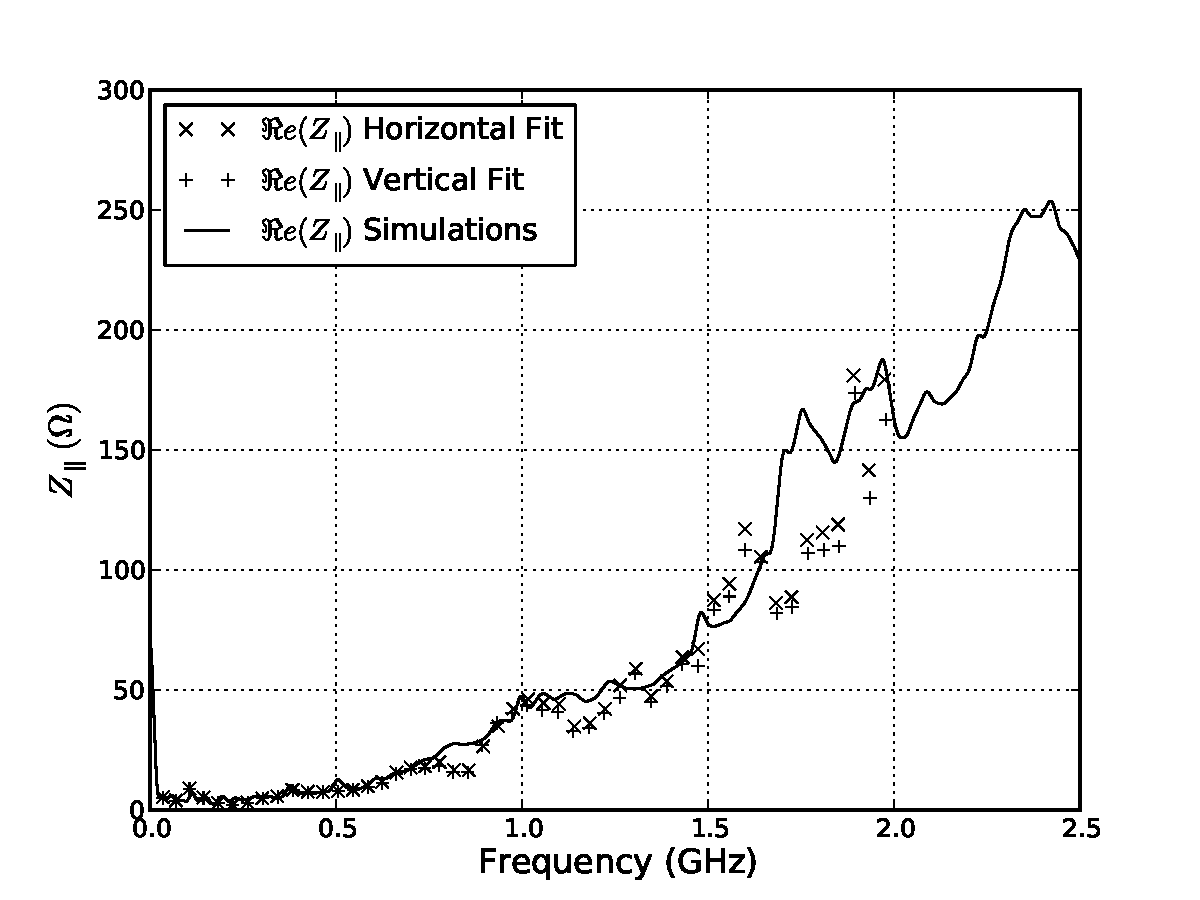
\includegraphics[width=0.8\textwidth]{LHC_MKI/figures/mki_15_sims_meas_long.pdf}
\end{center}
\label{fig:mki-15-longitudinal}
\caption{The longitudinal impedance of the LHC MKI acquired by measurements using the resonant coaxial wire method and time domain simulations using CST Particle Studio.}
\end{figure}

\begin{figure}
\subfigure[]{
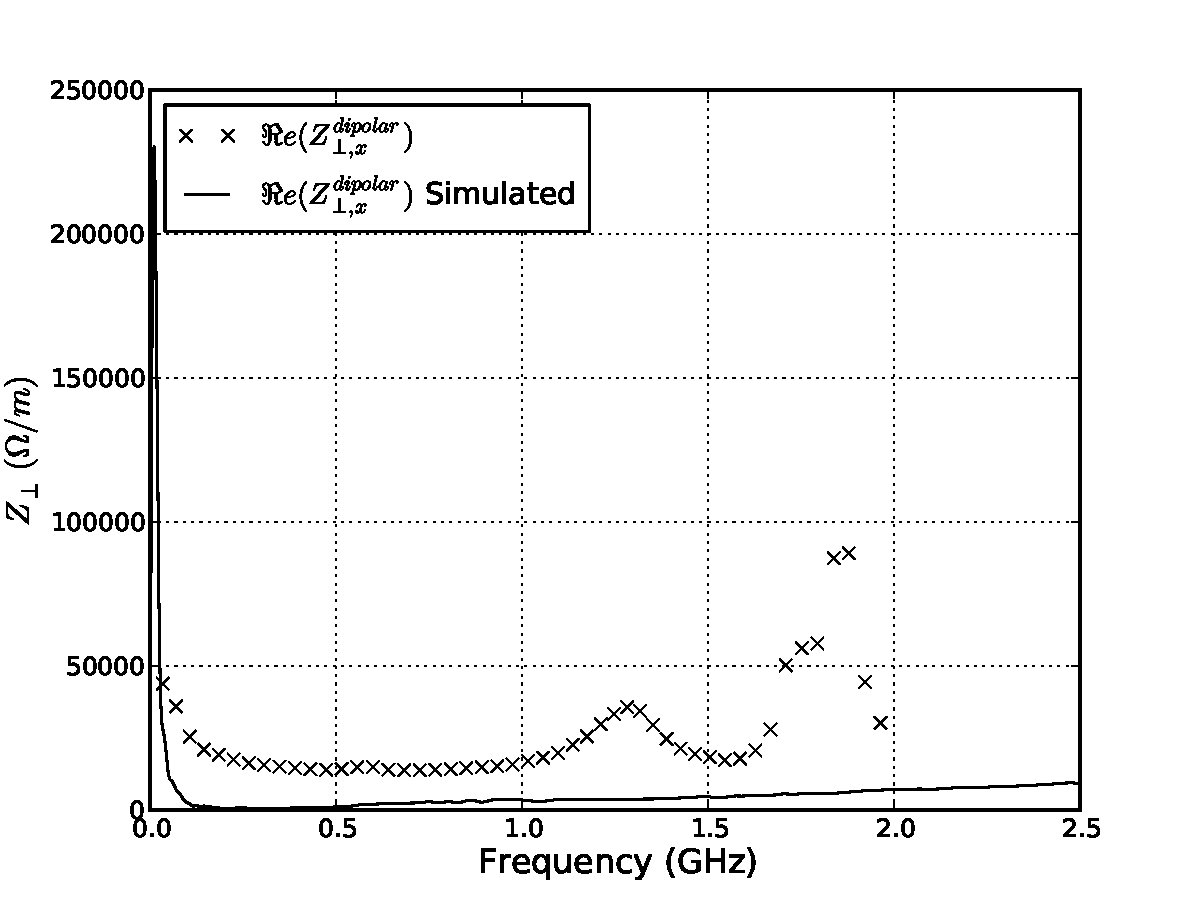
\includegraphics[width=0.45\textwidth]{LHC_MKI/figures/mki_15_sims_meas_dip_horz.pdf}
\label{fig:mki-15-horz-dipolar}
}
\subfigure[]{
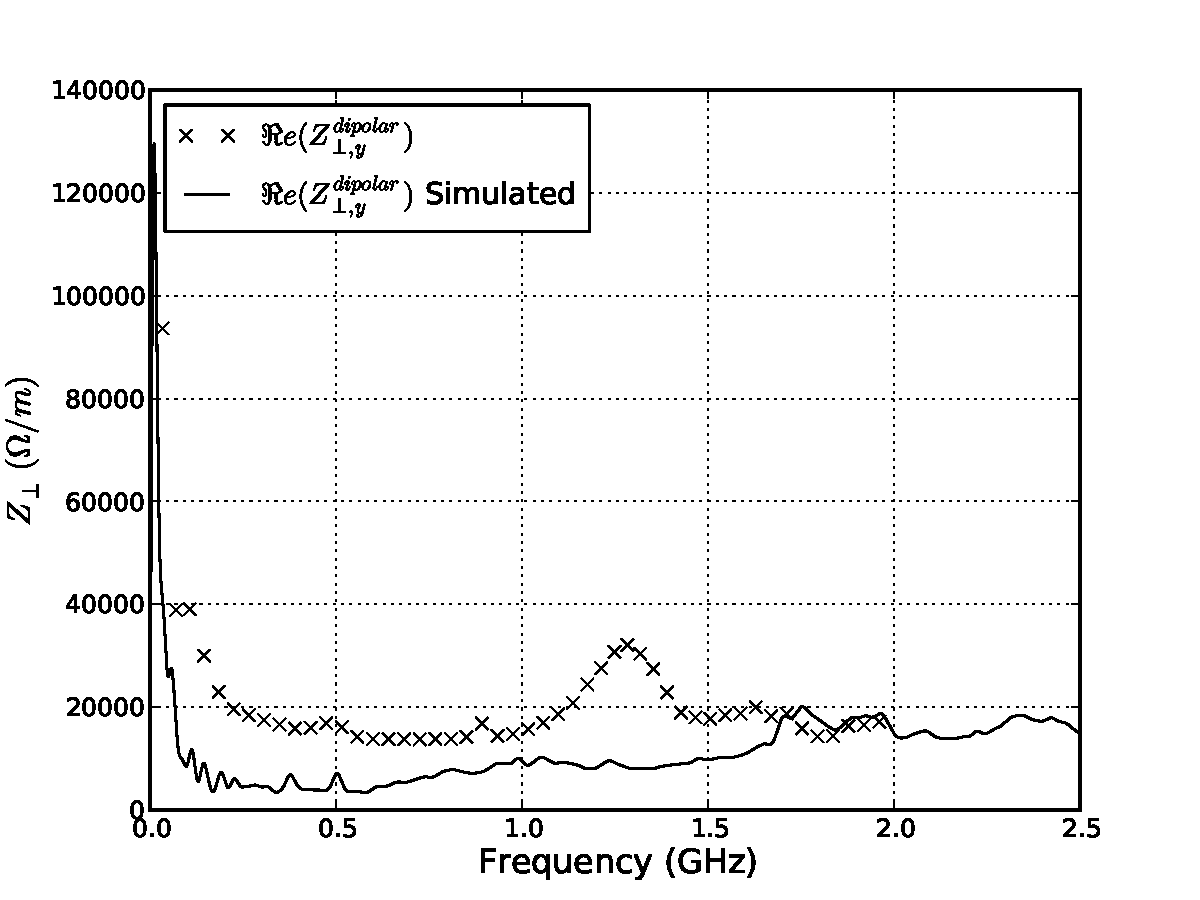
\includegraphics[width=0.45\textwidth]{LHC_MKI/figures/mki_15_sims_meas_dip_vert.pdf}
\label{fig:mki-15-vert-dipolar}
}
\label{fig:mki-15-dipolar}
\caption{The dipolar impedances of the LHC MKI acquired by measurements using the resonant coaxial wire method and time domain simulations using CST Particle Studio. \ref{fig:mki-15-horz-dipolar} shows the horizontal dipolar impedance, and \ref{fig:mki-15-vert-dipolar} the vertical dipolar impedance}
\end{figure}

\begin{figure}
\begin{center}
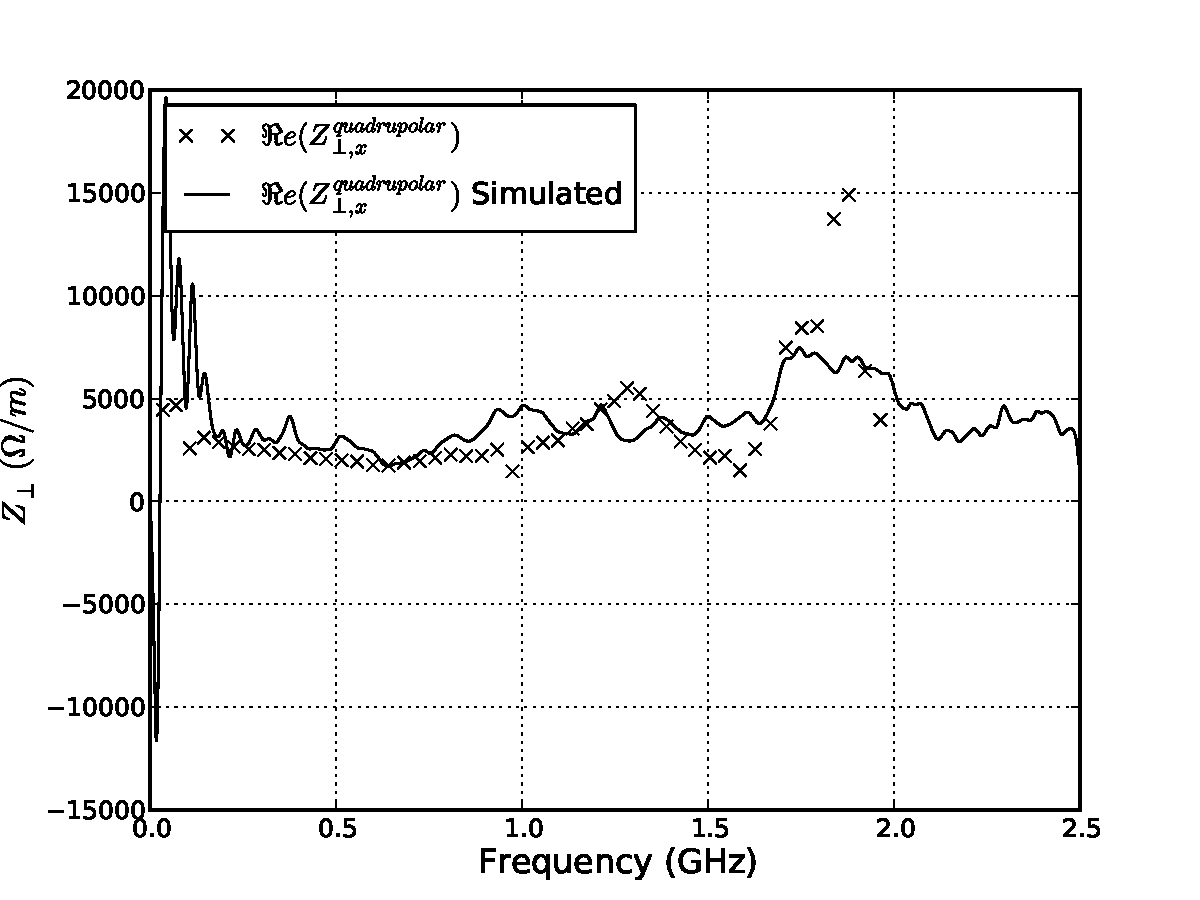
\includegraphics[width=0.7\textwidth]{LHC_MKI/figures/mki_15_sims_meas_quad_horz.pdf}
\end{center}
\label{fig:mki-15-quadrupolar}
\caption{The quadrupolar impedances of the LHC MKI acquired by measurements using the resonant coaxial wire method and time domain simulations using CST Particle Studio.}
\end{figure}

\begin{figure}
\begin{center}
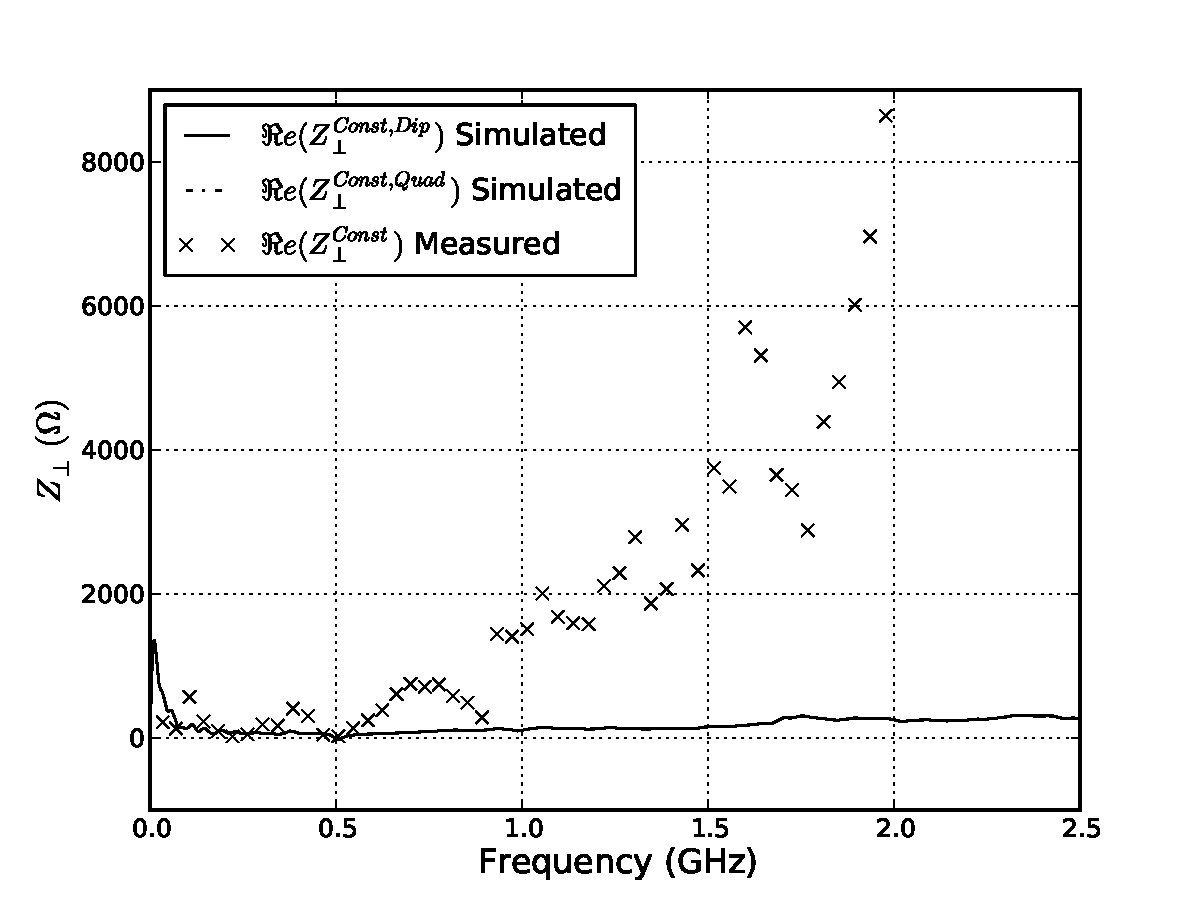
\includegraphics[width=0.7\textwidth]{LHC_MKI/figures/mki_15_sims_meas_const.pdf}
\end{center}
\label{fig:mki-15-constant}
\caption{The constant transverse impedances of the LHC MKI acquired by measurements using the resonant coaxial wire method and time domain simulations using CST Particle Studio.}
\end{figure}


It can be seen that there is generally good agreement between the measurements and simulations in all planes. In particular the agreement for the real component of the longitudinal impedance between measurements and simulations is exceptionally good below 1.5GHz. This is considered an important verification of the simulation model as this is the impedance of greatest concern presently due to beam-induced heating. Discrepencies can be seen in the longitudinal measurements above 1.5GHz - this is likely due to differences between the internal structure of the magnet and that represented by the simulation model.

In the transverse plane the dipolar impedance in both the vertical and horizontal plane shows good agreement between the simulations and the measurements. Likewise the agreement for the quadrupolar impedance is good over much of the frequency range, although the simulation and measurement results begin to diverge above 1.7GHz. The constant transverse term shows a good agreement up until $\approx$ 1GHz whereupon the results diverge. This is due to the sentivity of these results to the systematic and random errors in the measurement of the longitudinal impedance. The comparatively small longitudinal impedance measured in this instance leads to large errors in these results. 

\subsection{Beam Induced Heating Estimates for 15 Screen Conductors}

It can clearly be seen from the measurements of the real longitudinal impedance (\ref{fig:mki-15-longitudinal}) that there is a significant broadband impedance to the structure which could a cause of beam induced heating. This strongly indicates that the removal of the 9 screen conductors closest to te HV busbar has drastically decreased the screening of the ferrite from the beam image current.

To provide a first estimate of the expected heating of the MKI it is neccesary to estimate the power loss in the MKI. Taking the simulation impedance (due to allowing a finer resolution of frequency) the power is estimated using the broadband method of heat calculation given in Sec.~\ref{sec:beam-induced-heating}. For these calculations we consider the operational parameters for the 2012 proton run in the LHC, summarised in Tab.~\ref{tab:mki-beam-parameters}. Estimates for longitudinal profiles of gaussian, parabolic and cos$^{2}$ profiles assuming bunch lengths between 1.0 and 1.4ns are shown in Tab.~\ref{tab:mki-15-heating}. The thermal evolution of the MKI with this power load (assuming all the power is lost on the ferrite yoke for a worst case scenario) has by evaluated extensively by Garlasche et al \cite{Garlasche:2dHeat}, and has been found to be compatible with the measured temperature of the MKI thermal probes \cite{Barnes:mkiHeating}. As a response to this the interlock temperature was increased a number of times during 2011 and 2012 to take account of the expected internal temperature of the ferrite in relation to the measured temperature at the location of the temperature probes. In particular the measurement of the magnetic field parameters of the fired kicker (rise time, ripple and field strength) during the so called soft-start regime (firing the kicker with no beam) have provided accurate relations between the measured temperature and the ferrite yoke temperature \cite{Barnes:mkiHeating}.

\begin{table}
\label{tab:mki-beam-parameters}
\caption{The 2012 LHC operational parameters used for estimating the power loss in the MKI with 15 screen conductors.}
\begin{center}
\begin{tabular}{c | c | c}
Bunch Spacing & 50 & ns \\ \hline
Number of bunches & 1380 & \\ \hline
Particles per bunch & 1.7$\times 10^{11}$ & \\
\end{tabular}
\end{center}
\end{table}

\begin{table}
\label{tab:mki-15-heating}
\caption{Power loss estimates for the LHC-MKI with 15 screen conductors in the beam screen.}
\begin{center}
\begin{tabular}{c | c | c | c}
Bunch Length (ns) & $P_{loss, gaussian}$ & $P_{loss, parabolic}$ & $P_{loss, cos^{2}}$ \\ \hline
1.0 & 134 & 137 & 210 \\ \hline
1.1 & 113 & 115 & 171 \\ \hline
1.2 & 98 & 99 & 143 \\ \hline
1.3 & 86 & 88 & 123 \\ \hline
1.4 & 79 & 80 & 108 \\ \hline
\end{tabular}
\end{center}
\end{table}

It has thus been shown that the power loss due to the beam induced wakefields into the MKI can describe the temperature behaviour seen during 2011 and 2012 operation, giving us confidence in our understanding of the sources of and heating processes occuring within the MKI. To propose workable improvements to the beam screen, it is first neccesary to understand both the sources of the impedance due to the beam screen layout and the limitations that both manufacturability and the electrical potential build up on the screen conductors produces. In addition other methods of increasing decreasing both the power load and of improving the rate of cooling of the kicker are complementary avenues of study to reduce the problem of beam-induced heating in the MKIs, the problem ultimately being the high temperature of the ferrite yoke.

